\documentclass[12pt]{article}

%packages
%\usepackage{latexsym}
\usepackage{graphicx}
\usepackage{color}
\usepackage{amsmath}
\usepackage{dsfont}
\usepackage{placeins}
\usepackage{amssymb}
\usepackage{wasysym}
\usepackage{abstract}
\usepackage{hyperref}
\usepackage{etoolbox}
\usepackage{datetime}
\usepackage{xcolor}
\usepackage{alphalph}
\settimeformat{ampmtime}

%\usepackage{pstricks,pst-node,pst-tree}

%\usepackage{algpseudocode}
%\usepackage{amsthm}
%\usepackage{hyperref}
%\usepackage{mathrsfs}
%\usepackage{amsfonts}
%\usepackage{bbding}
%\usepackage{listings}
%\usepackage{appendix}
\usepackage[margin=1in]{geometry}
%\geometry{papersize={8.5in,11in},total={6.5in,9in}}
%\usepackage{cancel}
%\usepackage{algorithmic, algorithm}
\usepackage{fancyvrb}

\makeatletter
\def\maxwidth{ %
  \ifdim\Gin@nat@width>\linewidth
    \linewidth
  \else
    \Gin@nat@width
  \fi
}
\makeatother

\definecolor{fgcolor}{rgb}{0.345, 0.345, 0.345}
\newcommand{\hlnum}[1]{\textcolor[rgb]{0.686,0.059,0.569}{#1}}%
\newcommand{\hlstr}[1]{\textcolor[rgb]{0.192,0.494,0.8}{#1}}%
\newcommand{\hlcom}[1]{\textcolor[rgb]{0.678,0.584,0.686}{\textit{#1}}}%
\newcommand{\hlopt}[1]{\textcolor[rgb]{0,0,0}{#1}}%
\newcommand{\hlstd}[1]{\textcolor[rgb]{0.345,0.345,0.345}{#1}}%
\newcommand{\hlkwa}[1]{\textcolor[rgb]{0.161,0.373,0.58}{\textbf{#1}}}%
\newcommand{\hlkwb}[1]{\textcolor[rgb]{0.69,0.353,0.396}{#1}}%
\newcommand{\hlkwc}[1]{\textcolor[rgb]{0.333,0.667,0.333}{#1}}%
\newcommand{\hlkwd}[1]{\textcolor[rgb]{0.737,0.353,0.396}{\textbf{#1}}}%

\usepackage{framed}
\makeatletter
\newenvironment{kframe}{%
 \def\at@end@of@kframe{}%
 \ifinner\ifhmode%
  \def\at@end@of@kframe{\end{minipage}}%
  \begin{minipage}{\columnwidth}%
 \fi\fi%
 \def\FrameCommand##1{\hskip\@totalleftmargin \hskip-\fboxsep
 \colorbox{shadecolor}{##1}\hskip-\fboxsep
     % There is no \\@totalrightmargin, so:
     \hskip-\linewidth \hskip-\@totalleftmargin \hskip\columnwidth}%
 \MakeFramed {\advance\hsize-\width
   \@totalleftmargin\z@ \linewidth\hsize
   \@setminipage}}%
 {\par\unskip\endMakeFramed%
 \at@end@of@kframe}
\makeatother

\definecolor{shadecolor}{rgb}{.77, .77, .77}
\definecolor{messagecolor}{rgb}{0, 0, 0}
\definecolor{warningcolor}{rgb}{1, 0, 1}
\definecolor{errorcolor}{rgb}{1, 0, 0}
\newenvironment{knitrout}{}{} % an empty environment to be redefined in TeX

\usepackage{alltt}
\usepackage[T1]{fontenc}

\newcommand{\qu}[1]{``#1''}
\newcounter{probnum}
\setcounter{probnum}{1}

%create definition to allow local margin changes
\def\changemargin#1#2{\list{}{\rightmargin#2\leftmargin#1}\item[]}
\let\endchangemargin=\endlist 

%allow equations to span multiple pages
\allowdisplaybreaks

%define colors and color typesetting conveniences
\definecolor{gray}{rgb}{0.5,0.5,0.5}
\definecolor{black}{rgb}{0,0,0}
\definecolor{white}{rgb}{1,1,1}
\definecolor{blue}{rgb}{0.5,0.5,1}
\newcommand{\inblue}[1]{\color{blue}#1 \color{black}}
\definecolor{green}{rgb}{0.133,0.545,0.133}
\newcommand{\ingreen}[1]{\color{green}#1 \color{black}}
\definecolor{yellow}{rgb}{1,1,0}
\newcommand{\inyellow}[1]{\color{yellow}#1 \color{black}}
\definecolor{orange}{rgb}{0.9,0.649,0}
\newcommand{\inorange}[1]{\color{orange}#1 \color{black}}
\definecolor{red}{rgb}{1,0.133,0.133}
\newcommand{\inred}[1]{\color{red}#1 \color{black}}
\definecolor{purple}{rgb}{0.58,0,0.827}
\newcommand{\inpurple}[1]{\color{purple}#1 \color{black}}
\definecolor{backgcode}{rgb}{0.97,0.97,0.8}
\definecolor{Brown}{cmyk}{0,0.81,1,0.60}
\definecolor{OliveGreen}{cmyk}{0.64,0,0.95,0.40}
\definecolor{CadetBlue}{cmyk}{0.62,0.57,0.23,0}

%define new math operators
\DeclareMathOperator*{\argmax}{arg\,max~}
\DeclareMathOperator*{\argmin}{arg\,min~}
\DeclareMathOperator*{\argsup}{arg\,sup~}
\DeclareMathOperator*{\arginf}{arg\,inf~}
\DeclareMathOperator*{\convolution}{\text{\Huge{$\ast$}}}
\newcommand{\infconv}[2]{\convolution^\infty_{#1 = 1} #2}
%true functions

%%%% GENERAL SHORTCUTS

%shortcuts for pure typesetting conveniences
\newcommand{\bv}[1]{\boldsymbol{#1}}

%shortcuts for compound constants
\newcommand{\BetaDistrConst}{\dfrac{\Gamma(\alpha + \beta)}{\Gamma(\alpha)\Gamma(\beta)}}
\newcommand{\NormDistrConst}{\dfrac{1}{\sqrt{2\pi\sigma^2}}}

%shortcuts for conventional symbols
\newcommand{\tsq}{\tau^2}
\newcommand{\tsqh}{\hat{\tau}^2}
\newcommand{\sigsq}{\sigma^2}
\newcommand{\sigsqsq}{\parens{\sigma^2}^2}
\newcommand{\sigsqovern}{\dfrac{\sigsq}{n}}
\newcommand{\tausq}{\tau^2}
\newcommand{\tausqalpha}{\tau^2_\alpha}
\newcommand{\tausqbeta}{\tau^2_\beta}
\newcommand{\tausqsigma}{\tau^2_\sigma}
\newcommand{\betasq}{\beta^2}
\newcommand{\sigsqvec}{\bv{\sigma}^2}
\newcommand{\sigsqhat}{\hat{\sigma}^2}
\newcommand{\sigsqhatmlebayes}{\sigsqhat_{\text{Bayes, MLE}}}
\newcommand{\sigsqhatmle}[1]{\sigsqhat_{#1, \text{MLE}}}
\newcommand{\bSigma}{\bv{\Sigma}}
\newcommand{\bSigmainv}{\bSigma^{-1}}
\newcommand{\thetavec}{\bv{\theta}}
\newcommand{\thetahat}{\hat{\theta}}
\newcommand{\thetahatmle}{\hat{\theta}_{\mathrm{MLE}}}
\newcommand{\thetavechatmle}{\hat{\thetavec}_{\mathrm{MLE}}}
\newcommand{\muhat}{\hat{\mu}}
\newcommand{\musq}{\mu^2}
\newcommand{\muvec}{\bv{\mu}}
\newcommand{\muhatmle}{\muhat_{\text{MLE}}}
\newcommand{\lambdahat}{\hat{\lambda}}
\newcommand{\lambdahatmle}{\lambdahat_{\text{MLE}}}
\newcommand{\etavec}{\bv{\eta}}
\newcommand{\alphavec}{\bv{\alpha}}
\newcommand{\minimaxdec}{\delta^*_{\mathrm{mm}}}
\newcommand{\ybar}{\bar{y}}
\newcommand{\xbar}{\bar{x}}
\newcommand{\Xbar}{\bar{X}}
\newcommand{\phat}{\hat{p}}
\newcommand{\Phat}{\hat{P}}
\newcommand{\Zbar}{\bar{Z}}
\newcommand{\iid}{~{\buildrel iid \over \sim}~}
\newcommand{\inddist}{~{\buildrel ind \over \sim}~}
\newcommand{\approxdist}{~{\buildrel approx \over \sim}~}
\newcommand{\equalsindist}{~{\buildrel d \over =}~}
\newcommand{\loglik}[1]{\ell\parens{#1}}
\newcommand{\thetahatkminone}{\thetahat^{(k-1)}}
\newcommand{\thetahatkplusone}{\thetahat^{(k+1)}}
\newcommand{\thetahatk}{\thetahat^{(k)}}
\newcommand{\half}{\frac{1}{2}}
\newcommand{\third}{\frac{1}{3}}
\newcommand{\twothirds}{\frac{2}{3}}
\newcommand{\fourth}{\frac{1}{4}}
\newcommand{\fifth}{\frac{1}{5}}
\newcommand{\sixth}{\frac{1}{6}}

%shortcuts for vector and matrix notation
\newcommand{\A}{\bv{A}}
\renewcommand{\b}{\bv{b}}
\newcommand{\w}{\bv{w}}
\newcommand{\At}{\A^T}
\newcommand{\Ainv}{\inverse{\A}}
\newcommand{\B}{\bv{B}}
\newcommand{\K}{\bv{K}}
\newcommand{\Kt}{\K^T}
\newcommand{\Kinv}{\inverse{K}}
\newcommand{\Kinvt}{(\Kinv)^T}
\newcommand{\M}{\bv{M}}
\newcommand{\Bt}{\B^T}
\newcommand{\Q}{\bv{Q}}
\newcommand{\Qt}{\Q^T}
\newcommand{\R}{\bv{R}}
\newcommand{\Rt}{\R^T}
\newcommand{\Z}{\bv{Z}}
\newcommand{\X}{\bv{X}}
\newcommand{\Xsub}{\X_{\text{(sub)}}}
\newcommand{\Xsubadj}{\X_{\text{(sub,adj)}}}
\newcommand{\I}{\bv{I}}
\newcommand{\Y}{\bv{Y}}
\newcommand{\sigsqI}{\sigsq\I}
\renewcommand{\P}{\bv{P}}
\newcommand{\Psub}{\P_{\text{(sub)}}}
\newcommand{\Pt}{\P^T}
\newcommand{\Pii}{P_{ii}}
\newcommand{\Pij}{P_{ij}}
\newcommand{\IminP}{(\I-\P)}
\newcommand{\Xt}{X^\top}
\newcommand{\XtX}{\Xt X}
\newcommand{\XtXinv}{\parens{\Xt X}^{-1}}
\newcommand{\XtXinvXt}{\XtXinv\Xt}
\newcommand{\XXtXinvXt}{X\XtXinvXt}
\newcommand{\x}{\bv{x}}
\newcommand{\onevec}{\bv{1}}
\newcommand{\zerovec}{\bv{0}}
\newcommand{\oneton}{1, \ldots, n}
\newcommand{\yoneton}{y_1, \ldots, y_n}
\newcommand{\yonetonorder}{y_{(1)}, \ldots, y_{(n)}}
\newcommand{\Yoneton}{Y_1, \ldots, Y_n}
\newcommand{\iinoneton}{i \in \braces{\oneton}}
\newcommand{\onetom}{1, \ldots, m}
\newcommand{\jinonetom}{j \in \braces{\onetom}}
\newcommand{\xoneton}{x_1, \ldots, x_n}
\newcommand{\Xoneton}{X_1, \ldots, X_n}
\newcommand{\xt}{\x^T}
\newcommand{\y}{\bv{y}}
\newcommand{\yt}{\y^T}
\renewcommand{\c}{\bv{c}}
\newcommand{\ct}{\c^T}
\newcommand{\tstar}{\bv{t}^*}
\renewcommand{\u}{\bv{u}}
\renewcommand{\v}{\bv{v}}
\renewcommand{\a}{\bv{a}}
\newcommand{\s}{\bv{s}}
\newcommand{\yadj}{\y_{\text{(adj)}}}
\newcommand{\xjadj}{\x_{j\text{(adj)}}}
\newcommand{\xjadjM}{\x_{j \perp M}}
\newcommand{\yhat}{\hat{\y}}
\newcommand{\yhatsub}{\yhat_{\text{(sub)}}}
\newcommand{\yhatstar}{\yhat^*}
\newcommand{\yhatstarnew}{\yhatstar_{\text{new}}}
\newcommand{\z}{\bv{z}}
\newcommand{\zt}{\z^T}
\newcommand{\bb}{\bv{b}}
\newcommand{\bbt}{\bb^T}
\newcommand{\bbeta}{\bv{\beta}}
\newcommand{\beps}{\bv{\epsilon}}
\newcommand{\bepst}{\beps^T}
\newcommand{\e}{\bv{e}}
\newcommand{\Mofy}{\M(\y)}
\newcommand{\KofAlpha}{K(\alpha)}
\newcommand{\ellset}{\mathcal{L}}
\newcommand{\oneminalph}{1-\alpha}
\newcommand{\SSE}{\text{SSE}}
\newcommand{\SSEsub}{\text{SSE}_{\text{(sub)}}}
\newcommand{\MSE}{\text{MSE}}
\newcommand{\RMSE}{\text{RMSE}}
\newcommand{\SSR}{\text{SSR}}
\newcommand{\SST}{\text{SST}}
\newcommand{\JSest}{\delta_{\text{JS}}(\x)}
\newcommand{\Bayesest}{\delta_{\text{Bayes}}(\x)}
\newcommand{\EmpBayesest}{\delta_{\text{EmpBayes}}(\x)}
\newcommand{\BLUPest}{\delta_{\text{BLUP}}}
\newcommand{\MLEest}[1]{\hat{#1}_{\text{MLE}}}

%shortcuts for Linear Algebra stuff (i.e. vectors and matrices)
\newcommand{\twovec}[2]{\bracks{\begin{array}{c} #1 \\ #2 \end{array}}}
\newcommand{\threevec}[3]{\bracks{\begin{array}{c} #1 \\ #2 \\ #3 \end{array}}}
\newcommand{\fivevec}[5]{\bracks{\begin{array}{c} #1 \\ #2 \\ #3 \\ #4 \\ #5 \end{array}}}
\newcommand{\twobytwomat}[4]{\bracks{\begin{array}{cc} #1 & #2 \\ #3 & #4 \end{array}}}
\newcommand{\threebytwomat}[6]{\bracks{\begin{array}{cc} #1 & #2 \\ #3 & #4 \\ #5 & #6 \end{array}}}


%shortcuts for conventional compound symbols
\newcommand{\thetainthetas}{\theta \in \Theta}
\newcommand{\reals}{\mathbb{R}}
\newcommand{\complexes}{\mathbb{C}}
\newcommand{\rationals}{\mathbb{Q}}
\newcommand{\integers}{\mathbb{Z}}
\newcommand{\naturals}{\mathbb{N}}
\newcommand{\forallninN}{~~\forall n \in \naturals}
\newcommand{\forallxinN}[1]{~~\forall #1 \in \reals}
\newcommand{\matrixdims}[2]{\in \reals^{\,#1 \times #2}}
\newcommand{\inRn}[1]{\in \reals^{\,#1}}
\newcommand{\mathimplies}{\quad\Rightarrow\quad}
\newcommand{\mathlogicequiv}{\quad\Leftrightarrow\quad}
\newcommand{\eqncomment}[1]{\quad \text{(#1)}}
\newcommand{\limitn}{\lim_{n \rightarrow \infty}}
\newcommand{\limitN}{\lim_{N \rightarrow \infty}}
\newcommand{\limitd}{\lim_{d \rightarrow \infty}}
\newcommand{\limitt}{\lim_{t \rightarrow \infty}}
\newcommand{\limitsupn}{\limsup_{n \rightarrow \infty}~}
\newcommand{\limitinfn}{\liminf_{n \rightarrow \infty}~}
\newcommand{\limitk}{\lim_{k \rightarrow \infty}}
\newcommand{\limsupn}{\limsup_{n \rightarrow \infty}}
\newcommand{\limsupk}{\limsup_{k \rightarrow \infty}}
\newcommand{\floor}[1]{\left\lfloor #1 \right\rfloor}
\newcommand{\ceil}[1]{\left\lceil #1 \right\rceil}

%shortcuts for environments
\newcommand{\beqn}{\vspace{-0.25cm}\begin{eqnarray*}}
\newcommand{\eeqn}{\end{eqnarray*}}
\newcommand{\bneqn}{\vspace{-0.25cm}\begin{eqnarray}}
\newcommand{\eneqn}{\end{eqnarray}}

%shortcuts for mini environments
\newcommand{\parens}[1]{\left(#1\right)}
\newcommand{\squared}[1]{\parens{#1}^2}
\newcommand{\tothepow}[2]{\parens{#1}^{#2}}
\newcommand{\prob}[1]{\mathbb{P}\parens{#1}}
\newcommand{\cprob}[2]{\prob{#1~|~#2}}
\newcommand{\littleo}[1]{o\parens{#1}}
\newcommand{\bigo}[1]{O\parens{#1}}
\newcommand{\Lp}[1]{\mathbb{L}^{#1}}
\renewcommand{\arcsin}[1]{\text{arcsin}\parens{#1}}
\newcommand{\prodonen}[2]{\bracks{\prod_{#1=1}^n #2}}
\newcommand{\mysum}[4]{\sum_{#1=#2}^{#3} #4}
\newcommand{\sumonen}[2]{\sum_{#1=1}^n #2}
\newcommand{\infsum}[2]{\sum_{#1=1}^\infty #2}
\newcommand{\infprod}[2]{\prod_{#1=1}^\infty #2}
\newcommand{\infunion}[2]{\bigcup_{#1=1}^\infty #2}
\newcommand{\infinter}[2]{\bigcap_{#1=1}^\infty #2}
\newcommand{\infintegral}[2]{\int^\infty_{-\infty} #2 ~\text{d}#1}
\newcommand{\supthetas}[1]{\sup_{\thetainthetas}\braces{#1}}
\newcommand{\bracks}[1]{\left[#1\right]}
\newcommand{\braces}[1]{\left\{#1\right\}}
\newcommand{\set}[1]{\left\{#1\right\}}
\newcommand{\abss}[1]{\left|#1\right|}
\newcommand{\norm}[1]{\left|\left|#1\right|\right|}
\newcommand{\normsq}[1]{\norm{#1}^2}
\newcommand{\inverse}[1]{\parens{#1}^{-1}}
\newcommand{\rowof}[2]{\parens{#1}_{#2\cdot}}

%shortcuts for functionals
\newcommand{\realcomp}[1]{\text{Re}\bracks{#1}}
\newcommand{\imagcomp}[1]{\text{Im}\bracks{#1}}
\newcommand{\range}[1]{\text{range}\bracks{#1}}
\newcommand{\colsp}[1]{\text{colsp}\bracks{#1}}
\newcommand{\rowsp}[1]{\text{rowsp}\bracks{#1}}
\newcommand{\tr}[1]{\text{tr}\bracks{#1}}
\newcommand{\rank}[1]{\text{rank}\bracks{#1}}
\newcommand{\proj}[2]{\text{Proj}_{#1}\bracks{#2}}
\newcommand{\projcolspX}[1]{\text{Proj}_{\colsp{\X}}\bracks{#1}}
\newcommand{\median}[1]{\text{median}\bracks{#1}}
\newcommand{\mean}[1]{\text{mean}\bracks{#1}}
\newcommand{\dime}[1]{\text{dim}\bracks{#1}}
\renewcommand{\det}[1]{\text{det}\bracks{#1}}
\newcommand{\expe}[1]{\mathbb{E}\bracks{#1}}
\newcommand{\expeabs}[1]{\expe{\abss{#1}}}
\newcommand{\expesub}[2]{\mathbb{E}_{#1}\bracks{#2}}
\newcommand{\indic}[1]{\mathds{1}_{#1}}
\newcommand{\var}[1]{\mathbb{V}\text{ar}\bracks{#1}}
\newcommand{\cov}[2]{\mathbb{C}\text{ov}\bracks{#1, #2}}
\newcommand{\corr}[2]{\text{Corr}\bracks{#1, #2}}
\newcommand{\se}[1]{\mathbb{S}\text{E}\bracks{#1}}
\newcommand{\seest}[1]{\hat{\mathbb{S}\text{E}}\bracks{#1}}
\newcommand{\bias}[1]{\text{Bias}\bracks{#1}}
\newcommand{\derivop}[2]{\dfrac{\text{d}}{\text{d} #1}\bracks{#2}}
\newcommand{\partialop}[2]{\dfrac{\partial}{\partial #1}\bracks{#2}}
\newcommand{\secpartialop}[2]{\dfrac{\partial^2}{\partial #1^2}\bracks{#2}}
\newcommand{\mixpartialop}[3]{\dfrac{\partial^2}{\partial #1 \partial #2}\bracks{#3}}

%shortcuts for functions
\renewcommand{\exp}[1]{\mathrm{exp}\parens{#1}}
\renewcommand{\cos}[1]{\text{cos}\parens{#1}}
\renewcommand{\sin}[1]{\text{sin}\parens{#1}}
\newcommand{\sign}[1]{\text{sign}\parens{#1}}
\newcommand{\are}[1]{\mathrm{ARE}\parens{#1}}
\newcommand{\natlog}[1]{\ln\parens{#1}}
\newcommand{\oneover}[1]{\frac{1}{#1}}
\newcommand{\overtwo}[1]{\frac{#1}{2}}
\newcommand{\overn}[1]{\frac{#1}{n}}
\newcommand{\oneoversqrt}[1]{\oneover{\sqrt{#1}}}
\newcommand{\sqd}[1]{\parens{#1}^2}
\newcommand{\loss}[1]{\ell\parens{\theta, #1}}
\newcommand{\losstwo}[2]{\ell\parens{#1, #2}}
\newcommand{\cf}{\phi(t)}

%English language specific shortcuts
\newcommand{\ie}{\textit{i.e.} }
\newcommand{\AKA}{\textit{AKA} }
\renewcommand{\iff}{\textit{iff}}
\newcommand{\eg}{\textit{e.g.} }
\newcommand{\st}{\textit{s.t.} }
\newcommand{\wrt}{\textit{w.r.t.} }
\newcommand{\mathst}{~~\text{\st}~~}
\newcommand{\mathand}{~~\text{and}~~}
\newcommand{\ala}{\textit{a la} }
\newcommand{\ppp}{posterior predictive p-value}
\newcommand{\dd}{dataset-to-dataset}

%shortcuts for distribution titles
\newcommand{\logistic}[2]{\mathrm{Logistic}\parens{#1,\,#2}}
\newcommand{\bernoulli}[1]{\mathrm{Bernoulli}\parens{#1}}
\newcommand{\betanot}[2]{\mathrm{Beta}\parens{#1,\,#2}}
\newcommand{\stdbetanot}{\betanot{\alpha}{\beta}}
\newcommand{\multnormnot}[3]{\mathcal{N}_{#1}\parens{#2,\,#3}}
\newcommand{\normnot}[2]{\mathcal{N}\parens{#1,\,#2}}
\newcommand{\classicnormnot}{\normnot{\mu}{\sigsq}}
\newcommand{\stdnormnot}{\normnot{0}{1}}
\newcommand{\uniformdiscrete}[1]{\mathrm{Uniform}\parens{\braces{#1}}}
\newcommand{\uniform}[2]{\mathrm{U}\parens{#1,\,#2}}
\newcommand{\stduniform}{\uniform{0}{1}}
\newcommand{\geometric}[1]{\mathrm{Geometric}\parens{#1}}
\newcommand{\hypergeometric}[3]{\mathrm{Hypergeometric}\parens{#1,\,#2,\,#3}}
\newcommand{\exponential}[1]{\mathrm{Exp}\parens{#1}}
\newcommand{\gammadist}[2]{\mathrm{Gamma}\parens{#1, #2}}
\newcommand{\poisson}[1]{\mathrm{Poisson}\parens{#1}}
\newcommand{\binomial}[2]{\mathrm{Binomial}\parens{#1,\,#2}}
\newcommand{\negbin}[2]{\mathrm{NegBin}\parens{#1,\,#2}}
\newcommand{\rayleigh}[1]{\mathrm{Rayleigh}\parens{#1}}
\newcommand{\multinomial}[2]{\mathrm{Multinomial}\parens{#1,\,#2}}
\newcommand{\gammanot}[2]{\mathrm{Gamma}\parens{#1,\,#2}}
\newcommand{\cauchynot}[2]{\text{Cauchy}\parens{#1,\,#2}}
\newcommand{\invchisqnot}[1]{\text{Inv}\chisq{#1}}
\newcommand{\invscaledchisqnot}[2]{\text{ScaledInv}\ncchisq{#1}{#2}}
\newcommand{\invgammanot}[2]{\text{InvGamma}\parens{#1,\,#2}}
\newcommand{\chisq}[1]{\chi^2_{#1}}
\newcommand{\ncchisq}[2]{\chi^2_{#1}\parens{#2}}
\newcommand{\ncF}[3]{F_{#1,#2}\parens{#3}}

%shortcuts for PDF's of common distributions
\newcommand{\logisticpdf}[3]{\oneover{#3}\dfrac{\exp{-\dfrac{#1 - #2}{#3}}}{\parens{1+\exp{-\dfrac{#1 - #2}{#3}}}^2}}
\newcommand{\betapdf}[3]{\dfrac{\Gamma(#2 + #3)}{\Gamma(#2)\Gamma(#3)}#1^{#2-1} (1-#1)^{#3-1}}
\newcommand{\normpdf}[3]{\frac{1}{\sqrt{2\pi#3}}\exp{-\frac{1}{2#3}(#1 - #2)^2}}
\newcommand{\normpdfvarone}[2]{\dfrac{1}{\sqrt{2\pi}}e^{-\half(#1 - #2)^2}}
\newcommand{\chisqpdf}[2]{\dfrac{1}{2^{#2/2}\Gamma(#2/2)}\; {#1}^{#2/2-1} e^{-#1/2}}
\newcommand{\invchisqpdf}[2]{\dfrac{2^{-\overtwo{#1}}}{\Gamma(#2/2)}\,{#1}^{-\overtwo{#2}-1}  e^{-\oneover{2 #1}}}
\newcommand{\exponentialpdf}[2]{#2\exp{-#2#1}}
\newcommand{\poissonpdf}[2]{\dfrac{e^{-#1} #1^{#2}}{#2!}}
\newcommand{\binomialpdf}[3]{\binom{#2}{#1}#3^{#1}(1-#3)^{#2-#1}}
\newcommand{\rayleighpdf}[2]{\dfrac{#1}{#2^2}\exp{-\dfrac{#1^2}{2 #2^2}}}
\newcommand{\gammapdf}[3]{\dfrac{#3^#2}{\Gamma\parens{#2}}#1^{#2-1}\exp{-#3 #1}}
\newcommand{\cauchypdf}[3]{\oneover{\pi} \dfrac{#3}{\parens{#1-#2}^2 + #3^2}}
\newcommand{\Gammaf}[1]{\Gamma\parens{#1}}

%shortcuts for miscellaneous typesetting conveniences
\newcommand{\notesref}[1]{\marginpar{\color{gray}\tt #1\color{black}}}

%%%% DOMAIN-SPECIFIC SHORTCUTS

%Real analysis related shortcuts
\newcommand{\zeroonecl}{\bracks{0,1}}
\newcommand{\forallepsgrzero}{\forall \epsilon > 0~~}
\newcommand{\lessthaneps}{< \epsilon}
\newcommand{\fraccomp}[1]{\text{frac}\bracks{#1}}

%Bayesian related shortcuts
\newcommand{\yrep}{y^{\text{rep}}}
\newcommand{\yrepisq}{(\yrep_i)^2}
\newcommand{\yrepvec}{\bv{y}^{\text{rep}}}


%Probability shortcuts
\newcommand{\SigField}{\mathcal{F}}
\newcommand{\ProbMap}{\mathcal{P}}
\newcommand{\probtrinity}{\parens{\Omega, \SigField, \ProbMap}}
\newcommand{\convp}{~{\buildrel p \over \rightarrow}~}
\newcommand{\convLp}[1]{~{\buildrel \Lp{#1} \over \rightarrow}~}
\newcommand{\nconvp}{~{\buildrel p \over \nrightarrow}~}
\newcommand{\convae}{~{\buildrel a.e. \over \longrightarrow}~}
\newcommand{\convau}{~{\buildrel a.u. \over \longrightarrow}~}
\newcommand{\nconvau}{~{\buildrel a.u. \over \nrightarrow}~}
\newcommand{\nconvae}{~{\buildrel a.e. \over \nrightarrow}~}
\newcommand{\convd}{~{\buildrel \mathcal{D} \over \rightarrow}~}
\newcommand{\nconvd}{~{\buildrel \mathcal{D} \over \nrightarrow}~}
\newcommand{\withprob}{~~\text{w.p.}~~}
\newcommand{\io}{~~\text{i.o.}}

\newcommand{\Acl}{\bar{A}}
\newcommand{\ENcl}{\bar{E}_N}
\newcommand{\diam}[1]{\text{diam}\parens{#1}}

\newcommand{\taua}{\tau_a}

\newcommand{\myint}[4]{\int_{#2}^{#3} #4 \,\text{d}#1}
\newcommand{\laplacet}[1]{\mathscr{L}\bracks{#1}}
\newcommand{\laplaceinvt}[1]{\mathscr{L}^{-1}\bracks{#1}}
\renewcommand{\min}[1]{\text{min}\braces{#1}}
\renewcommand{\max}[1]{\text{max}\braces{#1}}

\newcommand{\Vbar}[1]{\bar{V}\parens{#1}}
\newcommand{\expnegrtau}{\exp{-r\tau}}

%%% problem typesetting
\definecolor{darkgrey}{rgb}{0.10,0.10,0.9}

\newcommand{\problem}[1]{\noindent \colorbox{black}{{\color{yellow} \large{\textsf{\textbf{Problem \arabic{probnum}}}}~}} \addtocounter{probnum}{1} \vspace{0.2cm} \\ \iftoggle{professormode}{}{\color{darkgrey}} #1}

\newcommand{\easysubproblem}[1]{\ingreen{\item} \iftoggle{professormode}{}{\color{darkgrey}} [easy] #1 \color{black} }
\newcommand{\intermediatesubproblem}[1]{\inorange{\item} \iftoggle{professormode}{}{\color{darkgrey}} [harder] #1 \color{black} }
\newcommand{\hardsubproblem}[1]{\inred{\item} \iftoggle{professormode}{}{\color{darkgrey}} [difficult] #1 \color{black} }
\newcommand{\extracreditsubproblem}[1]{\inpurple{\item} \iftoggle{professormode}{}{\color{darkgrey}} [E.C.] #1 \color{black} }


\newcommand{\spc}[1]{\iftoggle{professormode}{\\ \vspace{#1cm}}{\\ \vspace{-0.3cm}}}

\makeatletter
\newalphalph{\alphmult}[mult]{\@alph}{26}
\renewcommand{\labelenumi}{(\alphmult{\value{enumi}})}

\newcommand{\support}[1]{\text{Supp}\bracks{#1}}
\newcommand{\mode}[1]{\text{Mode}\bracks{#1}}
\newcommand{\IQR}[1]{\text{IQR}\bracks{#1}}
\newcommand{\quantile}[2]{\text{Quantile}\bracks{#1,\,#2}}


\newtoggle{professormode}
%\toggletrue{professormode} %STUDENTS: DELETE or COMMENT this line



\title{MATH 390.4 / 650.2 Spring 2018 Homework \#3t}

\author{Chaim Eisenbach} %STUDENTS: write your name here


\iftoggle{professormode}{
\date{Due 11:59PM Friday, March 23, 2018 under the door of KY604 \\ \vspace{0.5cm} \small (this document last updated \today ~at \currenttime)}
}

\renewcommand{\abstractname}{Instructions and Philosophy}

\begin{document}
\maketitle

\iftoggle{professormode}{
\begin{abstract}
The path to success in this class is to do many problems. Unlike other courses, exclusively doing reading(s) will not help. Coming to lecture is akin to watching workout videos; thinking about and solving problems on your own is the actual ``working out.''  Feel free to \qu{work out} with others; \textbf{I want you to work on this in groups.}

Reading is still \textit{required}. For this homework set, read about all the concepts introduced in class online e.g. multivariate least squares linear modeling, orthogonal projections, QR decomposition, etc. This is your responsibility to supplement in-class with your own readings. Also, read ch 2 in Silver and 2--4 in Finlay.

The problems below are color coded: \ingreen{green} problems are considered \textit{easy} and marked \qu{[easy]}; \inorange{yellow} problems are considered \textit{intermediate} and marked \qu{[harder]}, \inred{red} problems are considered \textit{difficult} and marked \qu{[difficult]} and \inpurple{purple} problems are extra credit. The \textit{easy} problems are intended to be ``giveaways'' if you went to class. Do as much as you can of the others; I expect you to at least attempt the \textit{difficult} problems. 

This homework is worth 100 points but the point distribution will not be determined until after the due date. See syllabus for the policy on late homework.

Up to 10 points are given as a bonus if the homework is typed using \LaTeX. Links to instaling \LaTeX~and program for compiling \LaTeX~is found on the syllabus. You are encouraged to use \url{overleaf.com}. If you are handing in homework this way, read the comments in the code; there are two lines to comment out and you should replace my name with yours and write your section. The easiest way to use overleaf is to copy the raw text from hwxx.tex \emph{and} preamble.tex into two new overleaf tex files with the same name. If you are asked to make drawings, you can take a picture of your handwritten drawing and insert them as figures or leave space using the \qu{$\backslash$vspace} command and draw them in after printing or attach them stapled.

The document is available with spaces for you to write your answers. If not using \LaTeX, print this document and write in your answers. I do not accept homeworks which are \textit{not} on this printout. Keep this first page printed for your records.

\end{abstract}

\thispagestyle{empty}
\vspace{1cm}
NAME: \line(1,0){380}
\clearpage
}

\problem{These are questions about Silver's book, chapter 2.}


\begin{enumerate}

\intermediatesubproblem{If one's goal is to fit a model for a phenomenon $y$, what is the difference between the approaches of the hedgehog and the fox? Answer using notation from class (i.e. $t ,f, g, h^*, \delta, \epsilon, e, t, z_1, \ldots, z_t, \mathbb{D}, \mathcal{H}, \mathcal{A}, \mathcal{X}, \mathcal{Y}, X, y, n, p, x_{\cdot 1}, \ldots, x_{\cdot p}, x_{1 \cdot}, \ldots, x_{n \cdot}$, etc.). Connecting this to the modeling framework should really make you think about what Tetlock's observation means for political and historical phenomena.}\spc{4} \\
For a fox there are multiple $x's$ that are closer to our $z's$. Also, they reduce our errors by having a larger data set and a more nuanced algorithm. As opposed to hedgehogs whose $x's$ may not be as close to our $z's$. Also Hedgehogs stick with one $\mathcal{A}$ while Fox's can adjust their $\mathcal{A}$ depending on new information to get a better $g$.\\

\easysubproblem{Why did Harry Truman like hedgehogs? Are there a lot of people that think this way?}\spc{4}\\

He wanted definite answers to issues. This can be seen in a lot of his policy moves. Such as dropping the atom bombs, the containment plan, the Korean war, union strikes etc. He wasn't interested in a less definitive more nuanced opinion. \\
Many people thing this way. It is easier to think of something in concrete terms than in more nuanced ones. BIG BOLD PREDICTIONS\\

\hardsubproblem{Why is it that the more education one acquires, the less accurate one's predictions become?}\spc{4}

They have more opportunities to permute and manipulate the information they have to confirm their biases.\\

\easysubproblem{Why are probabilistic classifiers (i.e. algorithms that output functions that return probabilities) better than vanilla classifiers (i.e. algorithms that only return the class label)? We will move in this direction in class soon.}\spc{4}

Returning a probability is better than returning a definitive answer. We want a range of possible outcomes, which would be a more honest expression of the uncertainty found in the real world. It would be foolish to pin things down to an exact number.\\
\end{enumerate}

\problem{These are questions about Finlay's book, chapter 2-4. We will hold off on chapter 1 until we cover probability estimation after midterm 2.}


\begin{enumerate}

\easysubproblem{What term did we use in class for \qu{behavioral (outome) data}?}\spc{0}

$Y$: output space.

\easysubproblem{Write about some reasons why data scientists implement models that are subpar in predictive performance (p27).}\spc{3}\\
There are business requirements and constraints that need to be taken into account. Sacrifice a small amount of predictive accuracy to ensure that business requirements are met. In a real business environment the bottom line comes before perfection.\\

\easysubproblem{In the first wine example, what is the outcome metric and what kind of supervised learning was employed?}\spc{0}\\
Weighted scores, they used a decision tree which is a typed of classification model.

\easysubproblem{In the second wine example, what is the outcome metric and kind of supervised learning was employed?}\spc{0}

A regression, profits are being measured.

\easysubproblem{In the third chapter, why is it that some organizations cannot use predictive modeling to improve their business?}\spc{3}\\
cultural norms. Organizations have a set way of doing things. Which is why Finlay prefers "embedded analytics" over an "analytics culture".

\easysubproblem{In the bankruptcy case, what is the problem with merely using $g$ to obtain a $\hat{y}$ without any other information from the model?}\spc{3}\\
The model to predict these didn't take into account how rare foreclosure actually is. They ignored the culture. They couldn't differentiate between a good model and good business.

\easysubproblem{Chapter 3 talks about using the model with human judgment. Under what circumstances is this beneficial? Answer using notation from class (i.e. $t ,f, g, h^*, \delta, \epsilon, e, t$, $z_1, \ldots, z_t, \mathbb{D}, \mathcal{H}, \mathcal{A}, \mathcal{X}, \mathcal{Y}, X, y, n, p, x_{\cdot 1}, \ldots, x_{\cdot p}, x_{1 \cdot}, \ldots, x_{n \cdot}$, etc.).}\spc{3}

With human judgment it is easier to get closer to $f$, to develop a better algorithm. To give greater weight to more important $x's$. 

\hardsubproblem{In Chapter 4 Finlay makes an interesting observation based on his experience in data science. He says most predictive models have $p \leq 30$. Why do you think this is? Discuss.}\spc{5}\\
Even though according to Silver it is important to look at many different causes for an event to make better and more accurate predictions. Finlay is telling us that once you surpass a certain number of variables you no longer have information useful enough to improve your algorithm or whatever you are trying to do. There is a limited number of really important factors in determining the cause of something.\\

\easysubproblem{He says there is \qu{almost always other data that could be acquired ... [which] doesn't always come for free}. The \qu{data} he is talking about here specifically means \qu{more predictors} i.e. increasing $p$. In what cases would someone be willing to pay for this data?}\spc{3}\\

Pre-sifted data save the time to find your own good data among all the useless data.
Predictive analytics is good business. An investment in good data can produce a more profitable business model. Having better data leads to a more accurate model.

\easysubproblem{Table 4 lists \qu{data types} about what type of observations?}\spc{1}
Behavior of interest. To predict burglary.

\easysubproblem{What type of data does he find in his experience to be the most important to predictive modeling? Why do you think this is so?}\spc{3}\\
Data about primary behavior. It predicts a certain pattern about ones behavior.
\easysubproblem{If $x_{\cdot 17}$ was age and $x_{\cdot 18}$ is age of spouse, what is the most likely reason why adding $x_{\cdot 18}$ to $\mathbb{D}$ not be fruitful for predictive ability?}\spc{3}

It will provide only incremental benefit to the model. If we know one spouses age we already have a pretty good picture of the range of the other spouses age. "If new data is highly correlated with existing data then it won't add much to the power of your predictions".

\hardsubproblem{What is the lifespan of a predictive model? Why does it not last forever? Answer using notation from class (i.e. $t ,f, g, h^*, \delta, \epsilon, e, t$, $z_1, \ldots, z_t, \mathbb{D}, \mathcal{H}, \mathcal{A}, \mathcal{X}, \mathcal{Y}, X, y, n, p$, $x_{\cdot 1}, \ldots, x_{\cdot p}, x_{1 \cdot}, \ldots, x_{n \cdot}$, etc.).}\spc{3}

Eventually reality veers away from our model. So our $x's$ are further away from our $z's$ which are different from the initial $z's$. Also, our $g$ strays away from $f$, maybe $f$ leaves our $\mathcal{H}$ entirely.
\hardsubproblem{What does \qu{large enough to representative of the full population} (p80) mean? Answer using notation from class (i.e. $t ,f, g, h^*, \delta, \epsilon, e, t$, $z_1, \ldots, z_t, \mathbb{D}, \mathcal{H}, \mathcal{A}, \mathcal{X}, \mathcal{Y}, X, y, n, p$, $x_{\cdot 1}, \ldots, x_{\cdot p}, x_{1 \cdot}, \ldots, x_{n \cdot}$, etc.).}\spc{3}\\
We need a $\mathbb{D}$ that encompasses enough X and Y to become closer to $t$. Essentially enough to get to a $\mathcal{H}$ that encompasses an $h^*$ that is close enough to an $f$ that is close enough to $t$. \\
\easysubproblem{Is there a hype about \qu{big data} i.e. including millions of observations instead of a few thousand? Discuss Finlay's opinion.}\spc{3}\\

According to Finlay data is only important if it's good data. Storage has become so cheap that there is a lot of useless data that needs to be sifted through.

\easysubproblem{What is Finlay's solution to \qu{overfitting} (p84)?}\spc{5}

It will be less likely to occur if there are large samples being used.

\end{enumerate}


\problem{These are questions about association and correlation.}


\begin{enumerate}

\easysubproblem{Give an example of two variables that are both correlated and associated by drawing a plot.}\spc{4}
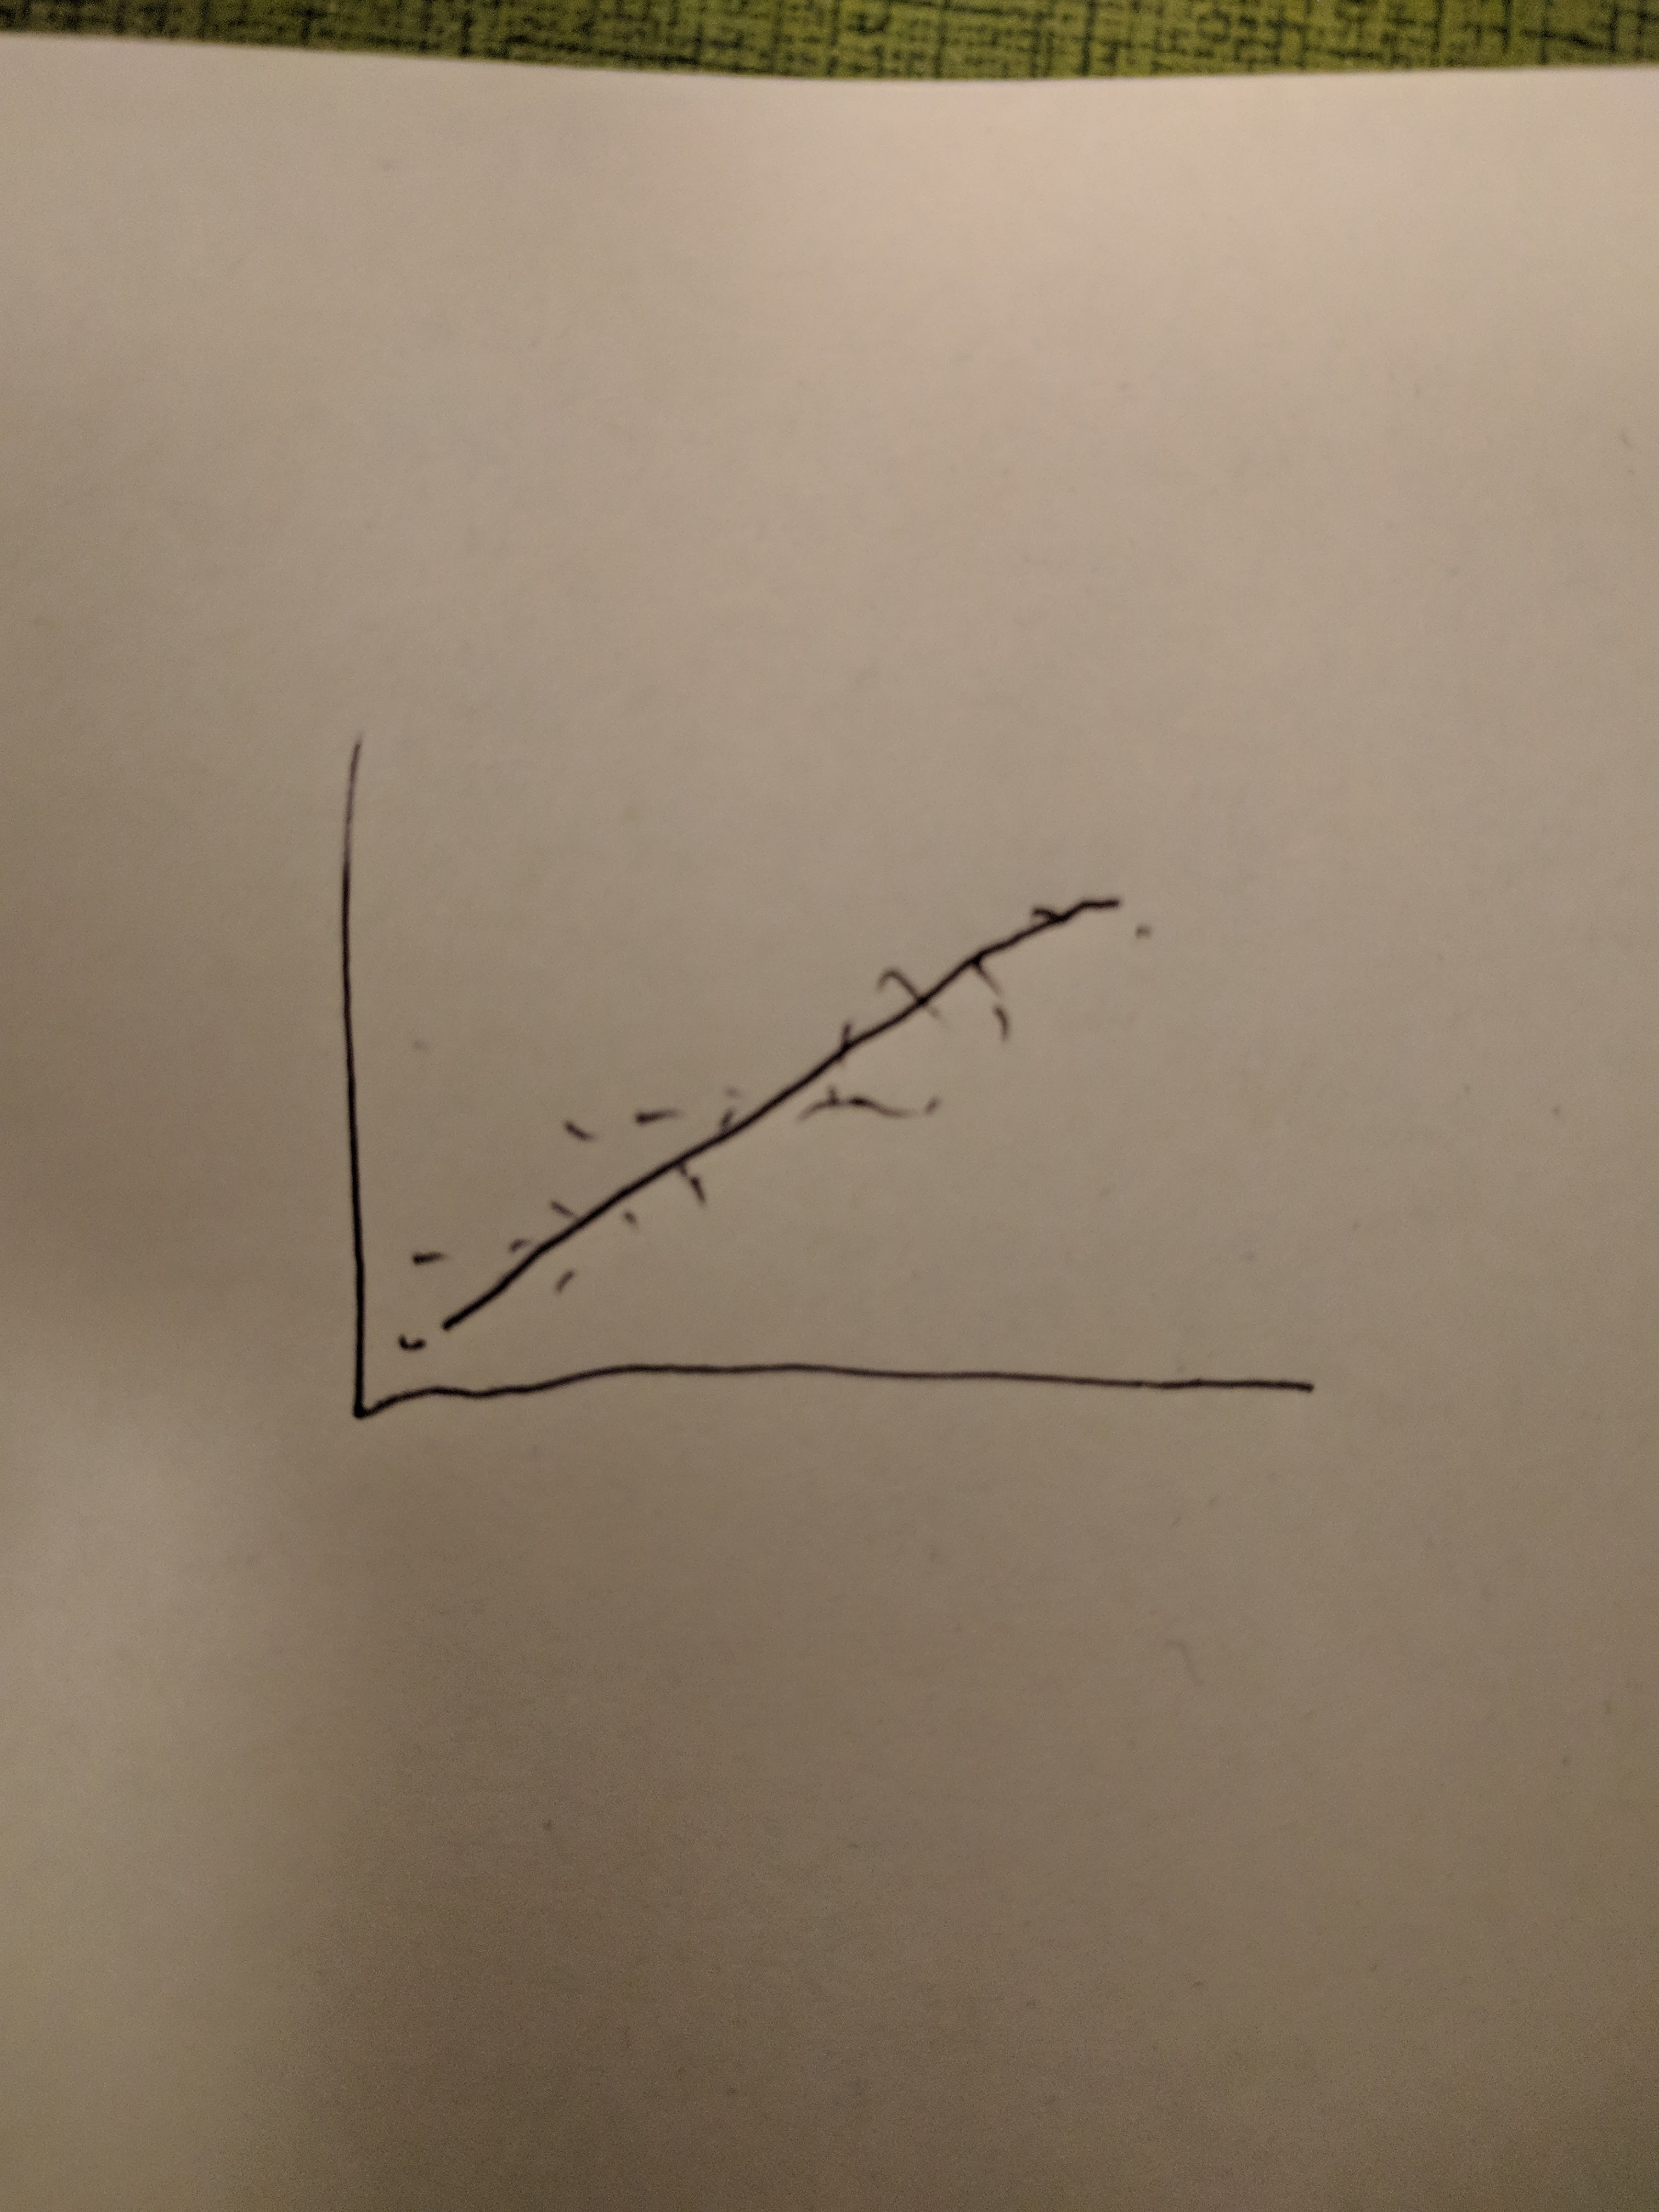
\includegraphics[scale =0.04]{corr.jpg}
\easysubproblem{Give an example of two variables that are not correlated but are associated by drawing a plot.}\spc{4}
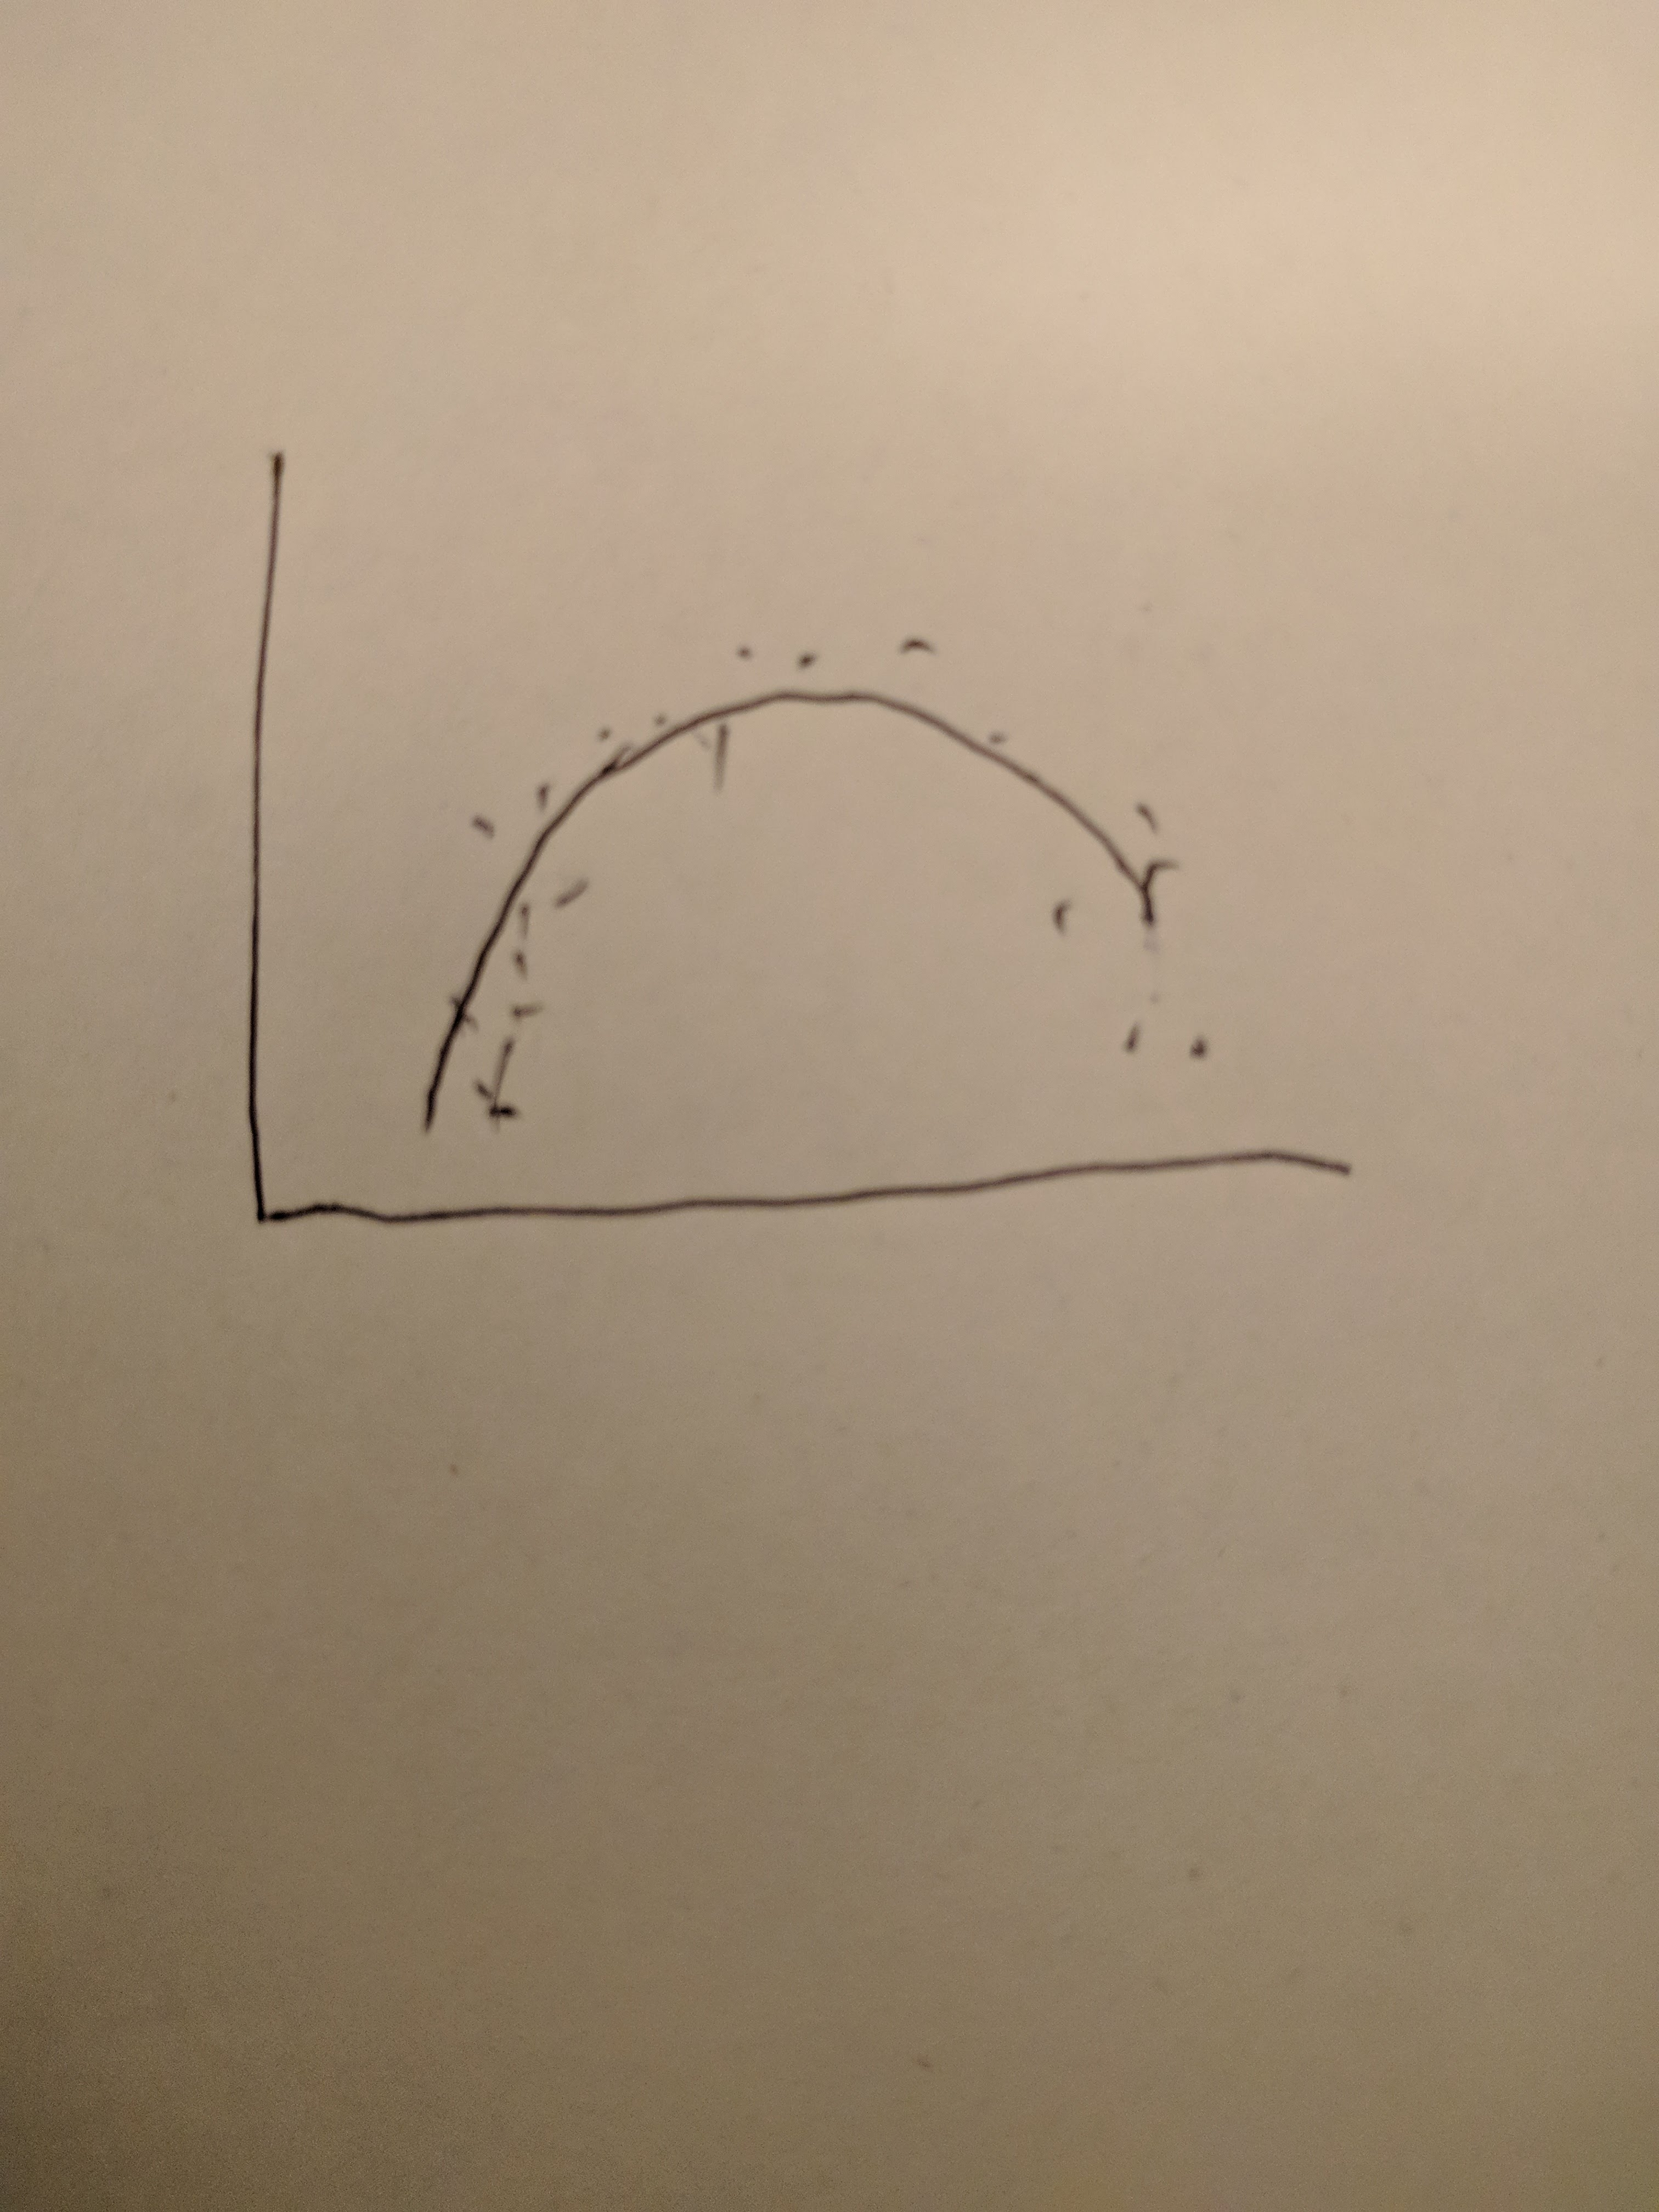
\includegraphics[scale =0.04]{assoc.jpg}
\easysubproblem{Give an example of two variables that are not correlated nor associated by drawing a plot.}\spc{4}
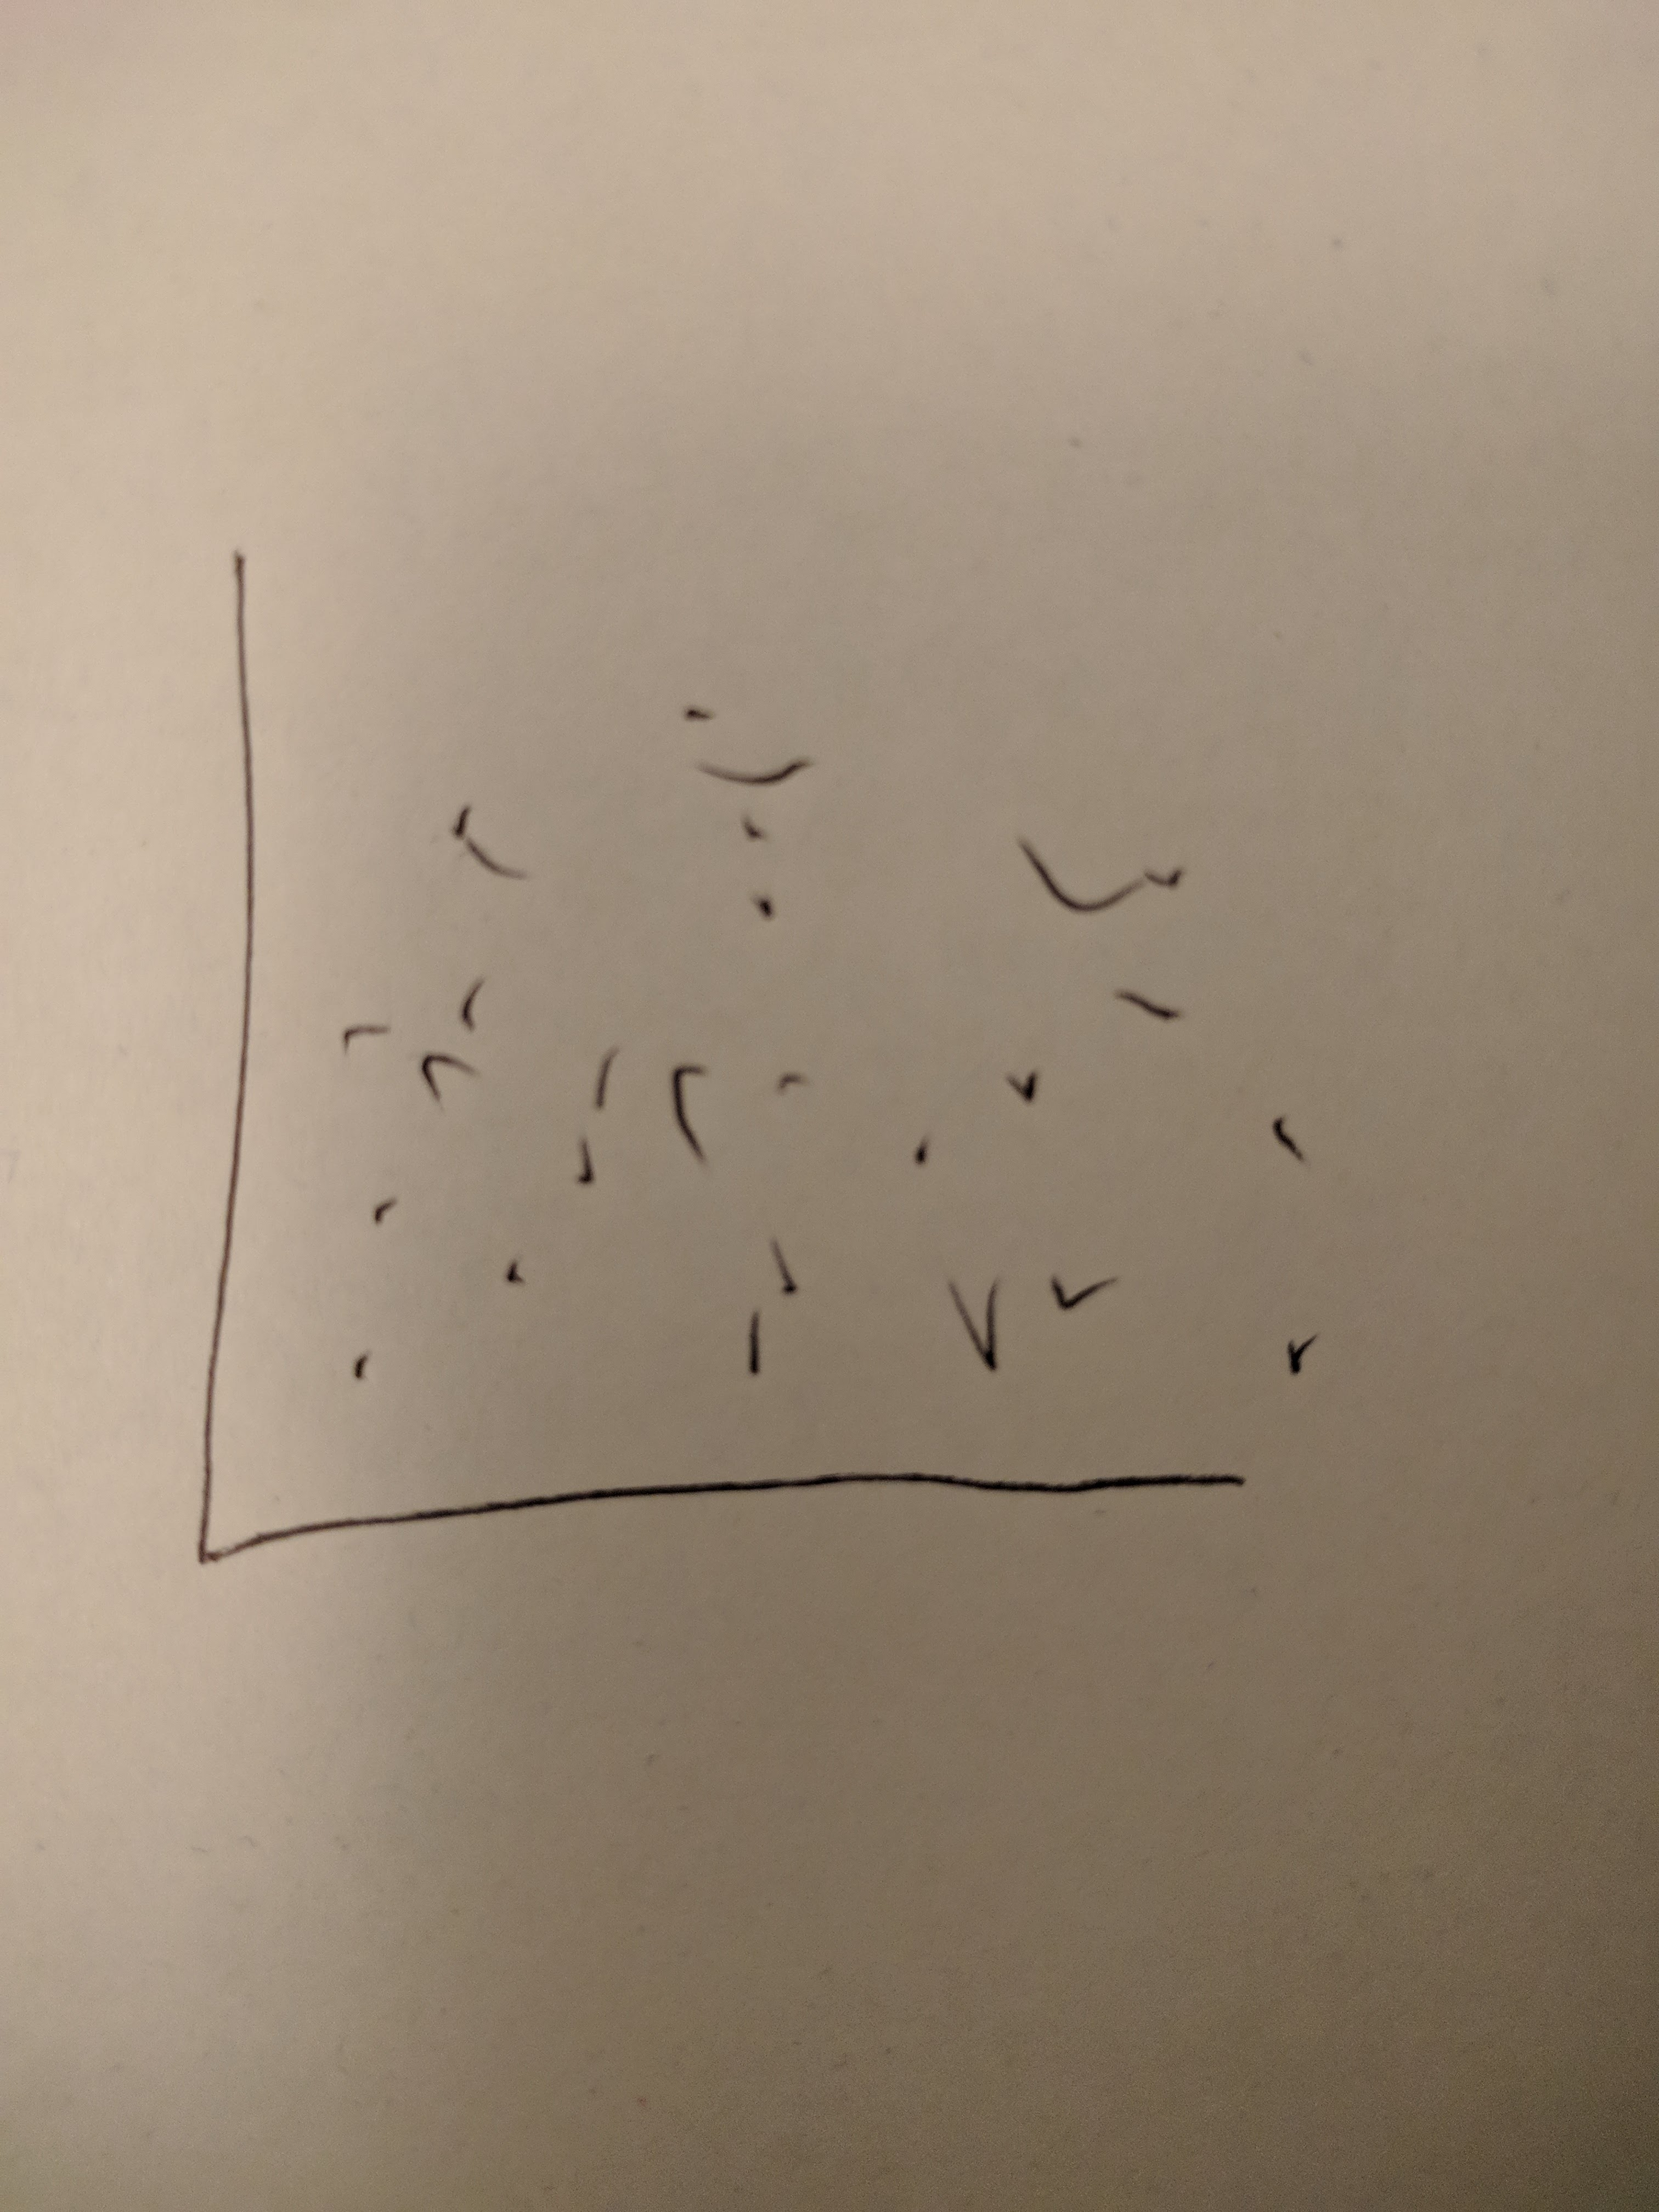
\includegraphics[scale =0.04]{non.jpg}
\easysubproblem{Can two variables be correlated but not associated? Explain.}\spc{4}
No. correlation $\in$ association.\\

\end{enumerate}

\problem{These are questions about multivariate linear model fitting using the least squares algorithm.}

\begin{enumerate}

\hardsubproblem{Derive $\partialop{\c}{\c^\top A \c}$ where $\c \in \reals^n$ and $A \in \reals^{n \times n}$ but \textit{not} symmetric. Get as far as you can.}\spc{8}\\
Looking at: ${\c^\top A \c}$ = $c_1(c_{11} + c_2a_{21} .... c_n a_{n1}) + c_2 (ca_{21} + ... + ca_{2n}) + c_n .....$\\
$\Rightarrow \sum\limits_{i=1}^n c_i \sum\limits_{j=1}^n c_ja_{ij}$\\
 $\partialop{\c_i}{\c^\top A \c} = \sum\limits_{j=1}^n c_ja_{ij} + c_ja_{ji}$

\easysubproblem{Given matrix $X \in \reals^{n \times (p+1)}$, full rank and first column consisting of the $\onevec_n$ vector, rederive the least squares solution $\b$ (the vector of coefficients in the linear model shipped in the prediction function $g$). No need to rederive the facts about vector derivatives.}\spc{10}

$\partialop{\w} {\vec{y}^\top \vec{y} - 2 \vec{w}^\top x^\top \vec{y} + \vec{w}^\top (x^\top x) \vec{w} } = 0_{p+1}^\top \Rightarrow (x^\top x)^{-1} x^\top x \vec{w} = (x^\top x)^{-1} x^\top \vec{y}$\\

$\vec{b} = (x^\top x)^{-1} x^\top \vec{y}$

\intermediatesubproblem{Consider the case where $p = 1$. Show that the solution for $\b$ you just derived is the same solution that we proved for simple regression in Lecture 8. That is, the first element of $\b$ is the same as $b_0 = \ybar - r \frac{s_y}{s_x}\xbar$ and the second element of $\b$ is $b_1 = r \frac{s_y}{s_x}$.} \spc{10}
$(X^\top X)^{-1} X^\top \vec{y} = \frac{1}{n \sum x_i^2 - n^2 \bar{x}^2}\begin{pmatrix}
\sum x_i^2 & -n\bar{x}\\ -n \bar{x} & n
\end{pmatrix}_ {(X^\top X)^{-1}} * \begin{pmatrix}
1 & . & . & . 1 \\ x_1 & .&.&.& x_n
\end{pmatrix}_{X^\top}
\begin{pmatrix}
y_1 \\ . \\ . \\.  \\ y_n
\end{pmatrix}_ {\vec{y}}$
\\

$=\frac{1}{n \sum x_i^2 - n^2 \bar{x}^2}\begin{pmatrix}
\sum x_i^2 & -n\bar{x}\\ -n \bar{x} & n
\end{pmatrix}_ {(X^\top X)^{-1}}
\begin{pmatrix}
n\bar{y}\\\sum y_i x_i
\end{pmatrix}_{X^\top \vec{y}}
= \frac{1}{n \sum x_i^2 - n^2 \bar{x}^2}
\begin{pmatrix}
n \bar{y} \sum x_i^2 & - n \sum y_i x_i\\ -n^2 \bar{x} \bar{y} & + n \sum y_i x_i
\end{pmatrix}\\
b_0 = \frac{\bar{y}(\sum x_i^2-n\bar{x}^2) - \bar{x} (\sum y_i x_i -n \bar{x}\bar{y} )}{\sum x_i^2 - n \bar{x}^2}\\
b_1 = \frac{\sum x_i y_i - n \bar{x} \bar{y}}{\sum x_i^2 -n\bar{x}^2}
$
\\

\easysubproblem{If $X$ is rank deficient, how can you solve for $\b$? Explain in English.} \spc{2}

Eliminate the linearly dependent vectors.

\hardsubproblem{Prove $\rank{X} =\rank{X^\top X}$.}\spc{6}

%Assume $\rank{X} < p+1$ and  $\rank{X^\top X} = p+1.\\ 
%\exists \vec{u} \neq 0 \in \reals^{p+1}$. Then $X \vec{u} = %\vec{0}_{p+1} \Rightarrow (X^\top X)$ not full rank $\Rightarrow$ %contradiction. 

Rank-Nullity Theorem: $\rank{X} = p+1 - \dim{(null(x))} = p+1 - \dim(null(X^\top X)) = \rank{X^\top X}$\\


\hardsubproblem{Given matrix $X \in \reals^{n \times (p+1)}$, full rank and first column consisting of the $\onevec_n$ vector, now consider cost multiples (\qu{weights}) $c_1, c_2, \ldots, c_n$ for each mistake $e_i$. As an example, previously the mistake for the 17th observation was $e_{17} := y_{17} - \hat{y}_{17}$ but now it would be $e_{17} := c_{17} (y_{17} - \hat{y}_{17})$.  Derive the weighted least squares solution $\b$. No need to rederive the facts about vector derivatives. Hints: (1) show that SSE is a quadratic form with the matrix $C$ in the middle (2) Split this matrix up into two pieces i.e. $C = C^{\half} C^{\half}$, distribute and then foil (3) note that a scalar value equals its own transpose and (4) use the vector derivative formulas.}\spc{20}\\
$\sum c_i (y_i - x_i w)^2\\ (y-xw)^\top c(y-xw)\\(y^\top cy - y^\top cxw - w^\top x^\top cy + w^\top x^\top cxw)\\$ taking the derivative we get $ 2(-x^\top cy + x^\top cxb) = 0\\ b= (x^\top cx)^{-1} x^\top cy$
\\
\hardsubproblem{If $p=1$, prove $r^2 = R^2$ i.e. the linear correlation is the same as proportion of sample variance explained in a least squares linear model.}\spc{6}\\
$R^2 = \frac{SSR}{SST} = \frac{\sum (\hat{y}- \bar{y})^2}{\sum (y - \bar{y})^2} \Rightarrow \frac{(\sum (x - \bar{x}) (y-\bar{y}))^2}{(\sum (x - \bar{x}))^2 (\sum(y-\bar{y}))^2} \Rightarrow \frac{Cov(x,y)^2}{S_x^2 S_y^2 } = r^2$
\\
\intermediatesubproblem{Prove that the point $<1,\xbar_1, \xbar_2, \ldots, \xbar_p, \bar{y}>$ is a point on the least squares linear solution.}\spc{13}\\
$\bar{y} = \frac{1}{n} \sum b_0 +b_1x_{i1}+...+b_nx_in$\\ 
$\bar{y} = b_0 +b_1\bar{x}_n +...+ b_n \bar{x}_n$\\
So the line goes through the averages of x and y.
\\

\end{enumerate}

\problem{These are questions related to the concept of orthogonal projection, QR decomposition and its relationship with least squares linear modeling.}

\begin{enumerate}

\easysubproblem{Consider least squares linear regression using a design matrix $X$ with rank $p + 1$. What are the degrees of freedom in the resulting model? What does this mean?}\spc{3}

$p + 1$ the degrees of freedom because it is the dimension of the column space of X. It's the independent pieces of data.

\intermediatesubproblem{If you are orthogonally projecting the vector $\y$ onto the column space of $X$ which is of rank $p + 1$, derive the formula for $\proj{\colsp{X}}{\y}$. Is this the same as the least squares solution?}\spc{6}\\
$\mathcal{X}$ = $\colsp{x}$\\ $\proj{\mathcal{X}}{\vec{\y}}$ = $X \vec{w}$\\ $X^\top (X \vec{w} - \vec{y}) = 0 \Leftarrow$ Because perpendicular. \\ $X^\top X \vec{w} = X^\top \vec{y}$\\ $\vec{w} = (X^\top X)^{-1} X^\top \vec{y}$\\ $X \vec{w} =X(X^\top X^{-1}) X^\top \vec{y}$\\ $\proj{\mathcal{X}}{\y} = X(X^\top X)^{-1} X^\top \vec{y}$

\hardsubproblem{We saw that the perceptron is an \textit{iterative algorithm}. This means that it goes through multiple iterations in order to converge to a closer and closer $\w$. Why not do the same with linear least squares regression? Consider the following. Regress $\y$ using $\X$ to get $\yhat$. This generates residuals $\e$ (the leftover piece of $\y$ that wasn't explained by the regression's fit, $\yhat$). Now try again! Regress $\e$ using $\X$ and then get new residuals $\e_{new}$. Would $\e_{new}$ be closer to $\zerovec_n$ than the first $\e$? That is, wouldn't this yield a better model on iteration \#2? Yes/no and explain.}\spc{10}
No, because the projection is the minimum error.

\intermediatesubproblem{Prove that $Q^\top = Q^{-1}$ where $Q$ is an orthonormal matrix such that $\colsp{Q} = \colsp{X}$ and $Q$ and $X$ are both matrices $\in \reals^{n \times (p+1)}$. Hint: this is purely a linear algebra exercise.}\spc{10}\\
 $Q^\top Q =\begin{pmatrix}
q_1^\top \\
.\\.\\.\\q_n^\top
\end{pmatrix}  
\begin{pmatrix} q_1&.&.&.&q_n 
\end{pmatrix} = I_{p+1}$ \\
$Q^\top Q = I$\\
So $Q^\top = Q^{-1}$

\intermediatesubproblem{Prove that the least squares projection $H = \XXtXinvXt$ is the same as $QQ^\top$.}\spc{10}\\
$X \in \reals ^{n\times n}$\\ $X = QR$, $Q^\top Q = I_n$, $R \in \reals^{n \times n}$\\ $(X^\top X)^{-1} X^\top = (R^\top Q^\top QR)^{-1}R^\top Q^\top = R^{-1}Q^\top$\\ $H = X(X^\top X)^{-1} X^\top = X R^{-1} Q^\top = QQ^\top $

\intermediatesubproblem{Prove that an orthogonal projection onto the $\colsp{Q}$ is the same as the sum of the projections onto each column of $Q$.}\spc{10}\\
$\proj{Q}{\vec{a}} = Q(Q^\top Q)^{-1} Q^\top \vec{a}= \sum\limits_{j=1}^{k} \frac{\vec{q_j}\vec{q_j}^\top}{\norm{\vec{q_j}}^2} = \sum\limits_{j=1}^{k} \vec{q_j}\vec{q_j}^\top \vec{a} = QQ^\top \vec{a}$
\\
\hardsubproblem{Trouble in paradise. Prove that the SSE of a multivariate linear least squares model always decreases (equivalently, $R^2$ always increases) upon the addition of a new independent predictor. Keep in mind this holds true even if this new predictor has no information about the true causal inputs to the phenomenon $y$.}\spc{12} \\

As SSR $\uparrow \Rightarrow$ SSE $\downarrow$ because SST = SSR + SSE\\
Adding a new piece, means rank is now $p+1+1$\\
SSR = $\sum\limits_{i=1}^n (\hat{y_i} -\bar{y})^2 = \sum y_i^2 - n \bar{y^2} = \sum\limits_{j=1}^{p+1} \norm{\proj{qj}{\vec{y}}}^2 + \norm{\proj{q_{new}}{\vec{y}}}^2$ \\
$\Rightarrow SSR_{new} \geq SSR \Rightarrow SSE_{new} \leq SSE \Rightarrow R_{new}^2 \geq R^2$\\


\intermediatesubproblem{Why is this a bad thing? Explain in English.}\spc{3}\\
$R^2$ can be made to look very good by adding more parameters without our model actually being better.\\


\extracreditsubproblem{Prove that $\rank{H} =\tr{H}$.}\spc{-0.5}
$\tr{H} = \tr{X(X^\top X)^{-1} X^{-1}} =\tr{X^\top X(X^\top X)^{-1}} = \tr{I_{p+1}} = p+1$
\end{enumerate}


\end{document}
